\section{Motivação}
\lstset{language=CFST, numbers=none}

\begin{frame}[fragile]{Contexto}
  \begin{itemize}
  \item Verificação estática da comunicação em programas concorrentes com troca de mensagens
    \newline
  \item Canais de comunicação governados por tipos de sessão
  \end{itemize}
\end{frame}

\begin{frame}[fragile]{Motivação}

  \begin{itemize}
  \item Exemplo: Transmitir uma lista num canal de comunicação
    \newline
    
\begin{lstlisting}  
data List = Nil | Cons Int List

type ListServer = &{
  Nil : end
  Cons : ?int . ListServer
}
\end{lstlisting}
  \end{itemize}
\end{frame}


\begin{frame}{Motivação}
  \begin{itemize}
    \item A sequência de operações num canal é definida por um autómato finito:
      \newline
      \usetikzlibrary{automata,positioning}
\tikzstyle{edge} = [draw,thick,->]
\begin{wrapfigure}{R}{0.35\textwidth}
%\begin{center}
  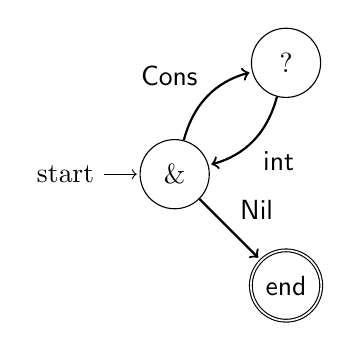
\begin{tikzpicture}[shorten >=1pt,node distance=2cm,on grid,auto] 
   \node[state,initial] (choice)   {$\&$}; 
   \node[state] (input) [above right=of choice] {$?$}; 
   \node[state,accepting] (end) [below right=of choice] {\textsf{end}}; 

   \path[edge] (choice) to[bend left] node {\textsf{Cons}} (input);
   \path[edge] (input) to[bend left] node {\textsf{int}} (choice);
   \path[edge] (choice) edge node {\textsf{Nil}} (end);
   
  \end{tikzpicture}
%\end{center}
\end{wrapfigure}

%%% Local Variables:
%%% mode: latex
%%% TeX-master: "cfst-inforum18"
%%% End:

    \item Linguagem regular: $(\textsf{\&Cons}\,\cdot\textsf{?Int})^*\cdot\textsf{\&Nil}$
      
  \end{itemize}

\end{frame}

\begin{frame}[fragile]{Motivação}
  \begin{itemize}
  \item E se o objetivo for transmitir uma árvore (num único canal)?
    \newline
    
    \lstinline"data Tree = Leaf | Node Int Tree Tree"
    \newline
  \item Objetivo: enviar sequências de \lstinline|Node|, \lstinline|Leaf| e \lstinline|Int|\\
  \newline
  \item Comunicação restrita ao envio de tipos básicos e sem passar novos canais

\item Os tipos de sessão devem garantir que as árvores estão bem formadas\\
      Exemplo: \lstinline|Node 2 Leaf Node 5 Leaf Leaf|\\
      Não exemplo: \lstinline|Node Leaf 2 Node Leaf|
\item Tipos de sessão independentes do contexto
  \end{itemize}
\end{frame}


%%% Local Variables:
%%% mode: latex
%%% TeX-master: "cfst"
%%% End: